\documentclass[twoside,openany,12pt]{beautynote} 
% Input Some Information of the doc
\doctitle{Complex Geometry}
\docsubtitle{\texorpdfstring{$L^2$}{} extension theorems with an optimal estimate and applications}
\dockeywords{\texorpdfstring{$L^2$}{} extension theorems with an optimal estimate and applications}
\date{\today\vfill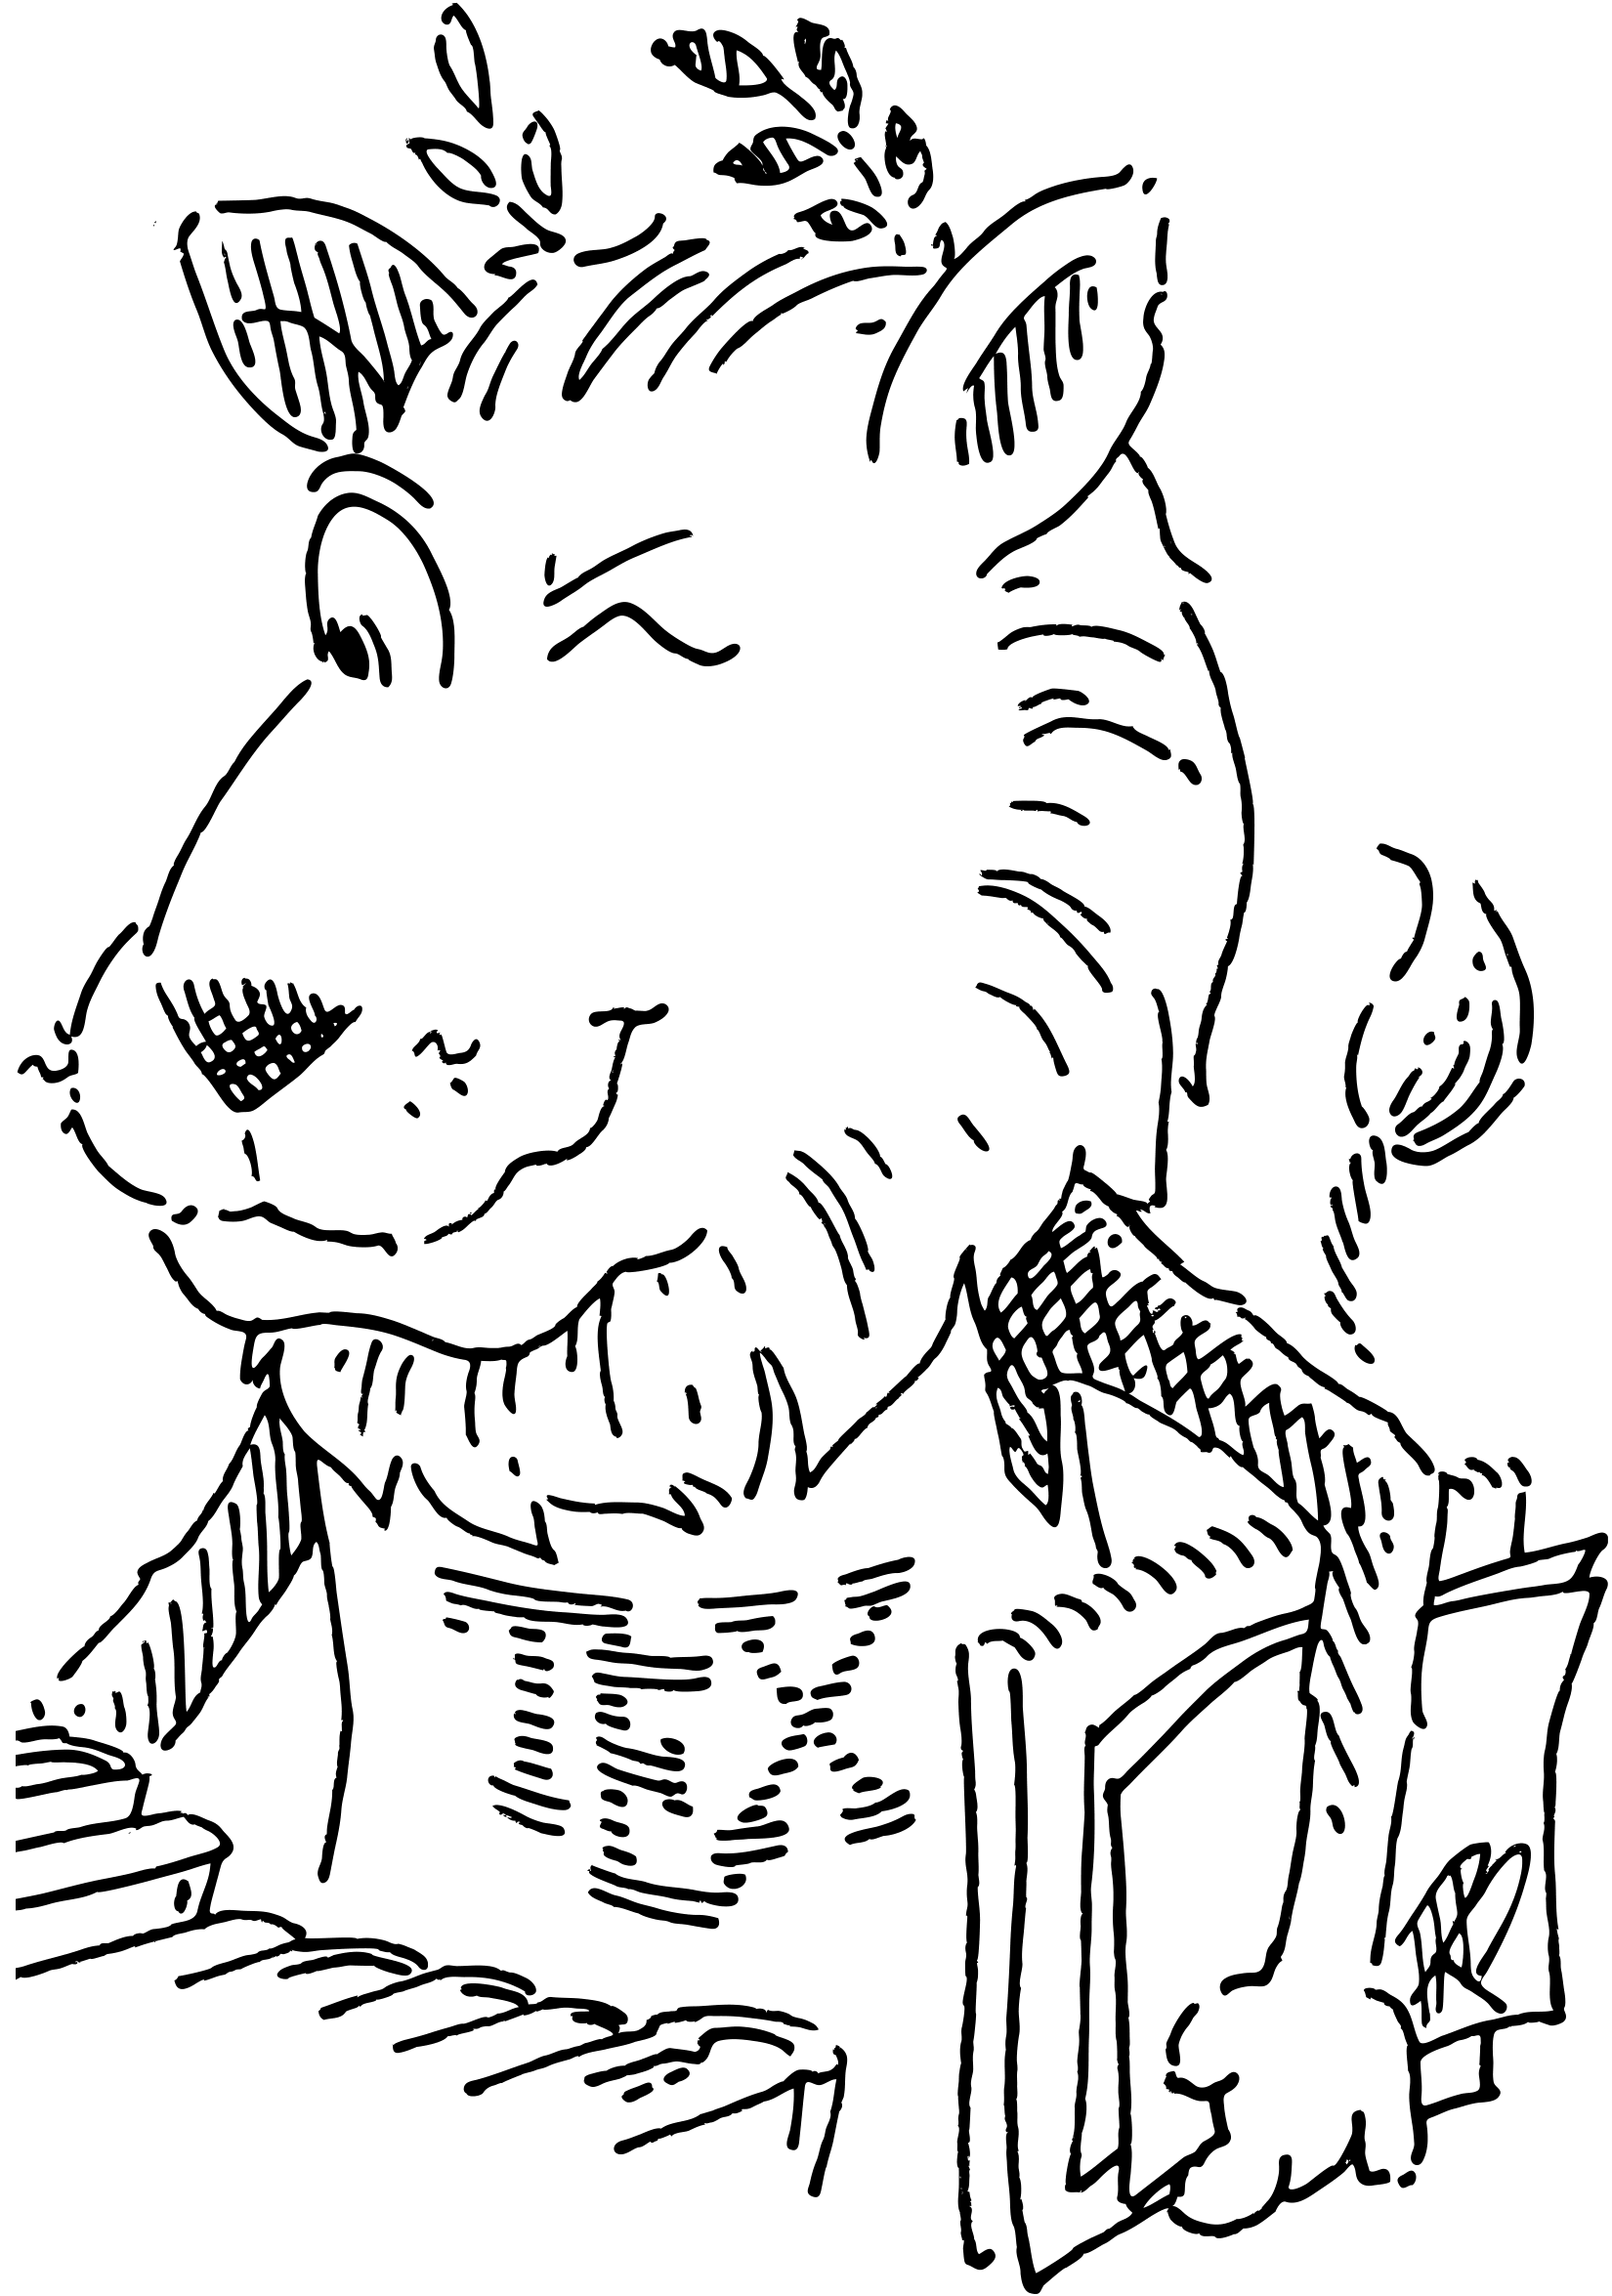
\includegraphics[width=0.15\textwidth]{titlepage.png}\\[.1em] \textsc{\large Beautynote}}
% Hyperref always required second to last.
\RequirePackage{hyperref}
\makeatletter
\hypersetup{%
    % hidelinks,
    pdfstartview=Fit,%
    pdfmenubar=true,%
    pdftoolbar=true,%
    bookmarksopen=false,%
    colorlinks=true,
    linkcolor=black,
    citecolor=purple,
    pdftitle={\@docsubtitle},%
    pdfauthor={\@author},%
    pdfsubject={\@doctitle},%
    pdflang={\languagename},%
    pdfkeywords={\@dockeywords},%
    pdfproducer={pdfTeX}}
\makeatother

% Cleveref as the last one.
\RequirePackage{cleveref}
%%%%%%%%%%%%%%%%%
\author{Ethan Lu}
\footext{}
\copyrightpage%
{Faculty of Pure Mathematics}% Your Faculty
{Sun Yat-Sen University}% Your University
{Press of Sun Yat-Sen University}% Your Publisher
{01A75, 00B50}% AMS
{Guang Zhou}% Your City
% If you do not want to fill one of the fields, please leave it like this: {}
\usepackage{appendix}
\usepackage{mathrsfs}
\usepackage{symbols}
\usepackage{bropd}
\usepackage{bm}
\usepackage{tabularray,booktabs}
\newcommand{\itbf}[1]{\textbf{\itshape #1}}\newcommand{\supp}{\operatorname{Supp}}\newcommand{\xu}{\sqrt{-1}}
\begin{document}
% --------------------------------- Titlepage -------------------------------- %
\maketitle\clearpage
% ------------------------------ Copyright-Page ------------------------------ %
\copyrights
\pagestyle{\auxsettings}
\makeatletter
\thispagestyle{copyright}
\ifdefempty{\@faculty}{}{\noindent {\large\textsc{\@faculty}} \\}
\ifdefempty{\@university}{}{{\large\textsc{\@university}} \\[1em]}
\ifdefempty{\@publisher}{}{\textit{Published by:} \@publisher \\}
\ifthenelse{\boolean{copyright}}{\textit{Copyright by:} \textsc{\templateauthor }\\}{} 
\ifdefempty{\@ams}{}{\textit{AMS Classification (2020):} \@ams.\\}
\vfill
\ifdefempty{\@city}{}{\noindent\@city, on \today\\}
\copyright\,\the\year\, \textsc{The Authors}
\doclicenseThis
\cleardoublepage
\makeatother
% ------------------------------ Copyright-Page ------------------------------ %
% ------------------------------------ Toc ----------------------------------- %
\tableofcontents
% ------------------------------- Main Contents ------------------------------ %
\pagestyle{\defaultsettings}
\chapter{Preliminaries}

\section{\texorpdfstring{$L^2$}{}-extension theorems with optimal constant}

\subsection{Some notations}
\newcommand{\tmop}[1]{\operatorname{#1}}
\NewTblrTheme{fancy}{
  \SetTblrStyle{firsthead}{font=\bfseries}
  \SetTblrStyle{firstfoot}{fg=purple2}
  \SetTblrStyle{middlefoot}{\itshape}
  \SetTblrStyle{caption-tag}{magenta2}
}
\begin{center}
\begin{tblr}[long,theme = fancy,
    caption = {Terminologies Interpretation},
    entry = {Interpretation},
    label = {tblr:Terminologies Interpretation 1},
    % note{a} = {第一个表注。},
    % note{$\dag$} = {第二个长长长长长长长的表注。},
    %   remark{Attention!} = {For any \textit{fine sheaf} $\sS$, one has $H^q(X,\sS)=0$ for $q\geqslant 1$.},
    % remark{来源} = {自力更生,自力更生,自力更生。},
    ]
    {
    colspec = {X|[dashed]X}, % 这是本来传入 tblr 的参数
    column{1}= {.25\linewidth,c},column{2}= {.7\linewidth}, rows = {m},
    width = \linewidth,
    row{odd} = {},
    % col{odd} = {gray9},
    row{1} = {1.3em,bg=cyan2,fg=white,font=\large\bfseries\sffamily},rowhead = 1, rowfoot = 1,
    row{even} = {brown9!60}, row{Z} = {bg=gray9,fg=red2},
    hline{1,2} = {0pt},
    hline{2,Y} = {dashed},
    hline{3-X} = {dashed,cyan2},
}
\textbf{Terminologies} & \textbf{Interpretations}\\ 
$M$ & complex $n$-dimensional manifold \\
  $S$ & a closed complex subvariety of $M$ \\ 
  $S_{reg}$ & the regular part of $S$ . \\ 
  $\dd V_M$ & a contionuous volume form on $M$\\  
$\#_A (S)$   & the set of such a class of the upper-semi-continuous (polar) function $\Psi\colon M\to [-\infty,A) , A\in (-\infty,+\infty]$ such that 
\begin{enumerate}
    \item $\Psi^{-1}(-\infty)\supset S$ and $\Psi^{-1}(-\infty)$  is a closed subset of $M$;\\[-1em]
    \item  if $S$ is $l$-dimensional around a point $x\in S_{reg}$, there exists a local coordinate $(z_1,\ldots,z_n)$ on a neighborhood $U$ of $x$ such that $z_{l+1}=\cdots=z_n=0$ on $S\cap U$ and      \[\sup_{U\backslash S}\abs{\Psi(z)-(n-l)\log \sum_{l+1}^n \abs{z_j}^2}<+\infty.\]
\end{enumerate}\\
$\Delta_{A,h,\delta}(S)$ & the subset of functions $\Psi$ in
$\#_{A}(S)$ which satisfies that both $he^{-\Psi}$ and
$he^{-(1+\delta)\Psi}$ are semi-positive in the sense of Nakano on
$M\setminus (X\cup S)$.\\

$\Delta_{A}(S)$ & the subset of plurisubharmonic functions
$\Psi$ in $\#_{A}(S)$\\
\itbf{Terminologies} & \itbf{Interpretations}\\ 
\end{tblr}
\end{center}


For each $\Psi\in\#_{A}(S)$, one can associate a positive measure
$dV_{M}[\Psi]$ on $S_{reg}$ as the minimum element of the partially
ordered set of positive measures $d\mu$ satisfying

$$\int_{S_{l}}fd\mu\geq\limsup_{t\to\infty}\frac{2(n-l)}
{\sigma_{2n-2l-1}}\int_{M}fe^{-\Psi}\mathbb{I}_{\{-1-t<\Psi<-t\}}dV_{M}$$
for any nonnegative continuous function $f$ with $\supp
f\subset\subset M$, where $\mathbb{I}_{\{-1-t<\Psi<-t\}}$ is the
characteristic function of the set $\{-1-t<\Psi<-t\}$. Here denote
by $S_{l}$ the $l$-dimensional component of $S_{reg}$, denote by
$\sigma_{m}$ the volume of the unit sphere in $\mathbb{R}^{m+1}$.

Let $\omega$ be a K\"{a}hler metric on $M\setminus (X\cup S)$, where
$X$ is a closed subset of $M$ such that $S_{sing}\subset X$
($S_{sing}$ is the singular part of $S$).

We can define measure $dV_{\omega}[\Psi]$ on $S\setminus X$ as the
minimum element of the partially ordered set of positive measures
$d\mu'$ satisfying
$$\int_{S_{l}}fd\mu'\geq\limsup_{t\to\infty}\frac{2(n-l)}
{\sigma_{2n-2l-1}}\int_{M\setminus (X\cup S)}fe^{-\Psi}\mathbb{I}_{\{-1-t<\Psi<-t\}}dV_{\omega}$$
for any nonnegative continuous function $f$ with
$\supp (f)\subset\subset M\setminus X$
(As $$\supp(\mathbb{I}_{\{-1-t<\Psi<-t\}})\cap \supp(f)\subset\subset M\setminus (X\cup S),$$
right hand side of the above inequality is well-defined).

Let $u$ be a continuous section of $K_{M}\otimes E$, where $E$ is a holomorphic vector bundle
equipped with a continuous metric $h$ on $M$.

We define
$$|u|^{2}_{h}|_{V}:=\frac{c_{n}h(e,e)v\wedge\bar{v}}{dV_{M}},$$
and
$$|u|^{2}_{h,\omega}|_{V}:=\frac{c_{n}h(e,e)v\wedge\bar{v}}{dV_{\omega}},$$
where $u|_{V}=v\otimes e$ for an open set $V\subset M\setminus (X\cup S)$, $v$ is a continuous section of
$K_{M}|_{V}$ and $e$ is a continuous
section of $E|_{V}$ (especially, we define
$$|u|^{2}|_{V}:=\frac{c_{n}u\wedge\bar{u}}{dV_{M}},$$
when $u$ is a continuous section of $K_{M}$). It is clear that
$|u|^{2}_{h}$ is independent of the choice of $V$.

The following argument shows a relationship between
$dV_{\omega}[\Psi]$ and $dV_{M}[\Psi]$ (resp. $dV_{\omega}$ and
$dV_{M}$), precisely
\begin{equation}
\label{equ:9.1}
\int_{M\setminus(X\cup S)}f|u|^{2}_{h,\omega}dV_{\omega}[\Psi]
=\int_{M\setminus(X\cup S)}f|u|^{2}_{h}dV_{M}[\Psi],
\end{equation}

\begin{equation}
\label{equ:9.2}
(resp.
\int_{M\setminus(X\cup S)}f|u|^{2}_{h,\omega}dV_{\omega}
=\int_{M\setminus(X\cup S)}f|u|^{2}_{h}dV_{M})
\end{equation}
where $f$ is a continuous function with compact support on $M\setminus X$.


Given $\delta>0$, let
\begin{enumerate}
  \item \itbf{Positivity:} $c_{A}(t)$ be a \textit{positive} function on
$(-A,+\infty)$ $(A\in(-\infty,+\infty))$
\item \itbf{smoothness:} $c_{A}(t)\in C^{\infty}((-A,+\infty))$
\item \itbf{Integrablity:} $\int_{-A}^{\infty}c_{A}(t)e^{-t}dt<\infty$
\item \itbf{Inequality:} \begin{equation}
\label{equ:c_A_delta}
\begin{split}
&\br{\frac{1}{\delta}c_{A}(-A)e^{A}+\int_{-A}^{t}c_{A}(t_{1})e^{-t_{1}}dt_{1}}^{2}>\\&c_{A}(t)e^{-t}
\br{\int_{-A}^{t}\br{\frac{1}{\delta}c_{A}(-A)e^{A}+\int_{-A}^{t_{2}}c_{A}(t_{1})e^{-t_{1}}dt_{1}}
dt_{2}+\frac{1}{\delta^{2}}c_{A}(-A)e^{A}},
\end{split}
\end{equation}
for any $t\in(-A,+\infty)$.
\end{enumerate}

\begin{definition}[Condition (ab)]
  Let $M$ be a complex manifold with a continuous volume form
  $dV_{M}$, and $S$ be a closed complex subvariety of $M$. We call
  $(M,S)$ satisfies condition $(ab)$ if $M$ and $S$ satisfy the
  following conditions:
  
  There exists a closed subset $X\subset M$ such that:
  
  $(a)$ $X$ is locally negligible with respect to $L^2$ holomorphic
  functions, i.e., for any local coordinate neighborhood $U\subset M$
  and for any $L^2$ holomorphic function $f$ on $U\setminus X$, there
  exists an $L^2$ holomorphic function $\tilde{f}$ on $U$ such that
  $\tilde{f}|_{U\setminus X}=f$ with the same $L^{2}$ norm.
  
  $(b)$ $M\setminus X$ is a Stein manifold which intersects with every component of $S$,
  such that $S_{sing}\subset X$.
  \end{definition}

If $c_{A}(t)e^{-t}$ is decreasing with respect to $t$, then
inequality \ref{equ:c_A_delta} holds.

We establish the following $L^{2}$ extension theorem with an optimal
estimate as follows:

\begin{theorem}[main theorem 1]\label{t:guan-zhou-semicontinu2}
Let $(M,S)$ satisfy condition $(ab)$,
$h$ be a smooth metric on a holomorphic vector bundle $E$ on $M$ with rank $r$.
Let $\Psi\in \#_{A}(S)\cap C^{\infty}(M\setminus S)$, which satisfies

\begin{enumerate}[label=\arabic*)]
  \item $he^{-\Psi}$ is semi-positive in the sense of Nakano on
$M\setminus (S\cup X)$ ($X$ is as in the definition of condition
$(ab)$),
\item there exists a continuous function $a(t)$ on $(-A,+\infty]$,
such that $0<a(t)\leq s(t)$ and
$a(-\Psi)\sqrt{-1}\Theta_{he^{-\Psi}}$ $+\sqrt{-1}\partial\bar\partial\Psi$
is semi-positive in the sense of Nakano on $M\setminus (S\cup X)$,
where $$s(t)=\frac{\int_{-A}^{t}(\frac{1}
{\delta}c_{A}(-A)e^{A}+\int_{-A}^{t_{2}}c_{A}(t_{1})e^{-t_{1}}dt_{1})dt_{2}+\frac{1}{\delta^{2}}c_{A}(-A)e^{A}}
{\frac{1}{\delta}c_{A}(-A)e^{A}+\int_{-A}^{t}c_{A}(t_{1})e^{-t_{1}}dt_{1}}.$$
\end{enumerate}

Then there exists a uniform constant $\bm{C}=1$, which is
optimal, such that, for any holomorphic section $f$ of $K_{M}\otimes
E|_{S}$ on $S$ satisfying
\begin{equation}
\label{equ:condition}
\sum_{k=1}^{n}\frac{\pi^{k}}{k!}\int_{S_{n-k}}|f|^{2}_{h}dV_{M}[\Psi]<\infty,
\end{equation}
there
exists a holomorphic section $F$ of $K_{M}\otimes E$ on $M$ satisfying $F = f$ on $ S$ and
\begin{equation}
\label{equ:optimal_delta}
\int_{M}c_{A}(-\Psi)|F|^{2}_{h}dV_{M}
\leq\bm{C}\br{\frac{1}{\delta}c_{A}(-A)e^{A}+\int_{-A}^{\infty}c_{A}(t)e^{-t}dt}
\sum_{k=1}^{n}\frac{\pi^{k}}{k!}\int_{S_{n-k}}|f|^{2}_{h}dV_{M}[\Psi],
\end{equation}
where $c_{A}(t)$ satisfies $c_{A}(-A)e^{A}:=\lim_{t\to -A^{+}}c_{A}(t)e^{-t}<\infty$ and $c_{A}(-A)e^{A}\neq0$.
\end{theorem}


\begin{remark}
  We need to clasify the following questions:
  \begin{enumerate}[label=\roman*)]
    \item What are the theorem say and its signification?
  \end{enumerate}
\end{remark}

Now we consider a useful and simpler class of functions as follows:

Let $c_{A}(t)$ be a positive function in $C^{\infty}((-A,+\infty))$
$(A\in(-\infty,+\infty])$, satisfying
$$\int_{-A}^{\infty}c_{A}(t)e^{-t}dt<\infty$$ and
\begin{equation}
\label{equ:c_A}
\left(\int_{-A}^{t}c_{A}(t_{1})e^{-t_{1}}dt_{1}\right)^{2}>c_{A}(t)e^{-t}
\int_{-A}^{t}\int_{-A}^{t_{2}}c_{A}(t_{1})e^{-t_{1}}dt_{1}dt_{2},
\end{equation}
for any $t\in(-A,+\infty)$.

When $c_{A}(t)e^{-t}$ is decreasing with respect to $t$ and $A$ is finite, inequality \ref{equ:c_A} holds.

For such a simpler and sufficiently useful class of functions, we
establish the following $L^2$ extension theorem with an optimal
estimate
%, whose simpler version was announced in \cite{guan-zhou13a}:
\begin{theorem}[The simple version of the main theorem]\label{t:guan-zhou-unify}
  Let $(M,S)$ satisfy condition $(ab)$, and $\Psi$ be a
plurisubharmonic function in $\Delta_{A}(S)\cap
C^{\infty}(M\setminus (S\cup X))$ ($X$ is as in the definition of
condition $(a,b)$), Let $h$ be a smooth metric on a holomorphic
vector bundle $E$ on $M$ with rank $r$, such that $he^{-\Psi}$ is
semi-positive in the sense of Nakano on $M\setminus (S\cup X)$,
(when $E$ is a line bundle, $h$ can be chosen as a semipositive
singular metric). Then there exists a uniform constant
$\mathbf{C}=1$, which is optimal, such that, for any holomorphic
section $f$ of $K_{M}\otimes E|_{S}$ on $S$ satisfying condition
\ref{equ:condition}  there exists a holomorphic section $F$ of
$K_{M}\otimes E$ on $M$ satisfying $F = f$ on $ S$ and
\begin{eqnarray*}
\int_{M}c_{A}(-\Psi)|F|^{2}_{h}dV_{M}
\leq\mathbf{C}\int_{-A}^{\infty}c_{A}(t)e^{-t}dt\sum_{k=1}^{n}\frac{\pi^{k}}{k!}\int_{S_{n-k}}|f|^{2}_{h}dV_{M}[\Psi].
\end{eqnarray*}
\end{theorem}

\subsection{Proof of Lemma 4.4}

\begin{lemma}[Lemma 4.4 \cite{Guan2015ASO}]
Let $\Delta$ be the unit disc and $\Delta_r$ be the disc with radius $r$. Then for any holomorphic function $f$ on $\Delta$, which satisfies $\int_\Delta \abs{f}^2 \dd \lambda<\infty$, we have a uniformly constant $C_r=\frac{1}{1-r^2}$, which is only dependent on $r$, such that \[\int_\Delta \abs{f}^2\dd \lambda\leq C_r \int_{\Delta\backslash \Delta_r}\abs{f}^2\dd \lambda,\]
where $\lambda$ is the Lebsgue measure on $\bC$.
\end{lemma}


\subsection{Proof of Lemma 4.5}

Let 
\[
  L^2_h(M):=\biggl\{\alpha\mid \alpha\in \Omega^{n,0}_M(E),\int_E \{\alpha,\alpha\}_h<\infty\biggr\}.
\]
where $\{\alpha,\alpha\}_h=:\abs{\alpha}_h^2 \dd V_M$.
\begin{proof}
  We can choose a covering $\left\{U_i\right\}_{i=1,2, \ldots}$ of $M$, which satisfies
  \begin{enumerate}[label=(\arabic*)]
    \item $U_i \subset \subset M$, and $\exists K_i \subset \subset U_i$, such that $\bigcup_{i=1}^{\infty} K_i=M$;
    \item $\left.E\right|_{U_i}$ is trivial with holomorphic basis $e_1^i, \ldots, e_r^i$;
    \item $\left.K_M\right|_{U_i}$ is trivial with holomorphic basis $v^i$.
  \end{enumerate}

Then we may write $\left.F_j\right|_{U_i}=f_{j, i}^k e_k^i \otimes v^i$, where $f_{j, i}^k$ are holomorphic functions on $U_i$. As $h$ is a Hermitian metric and $U_i \subset \subset M$, there exists a constant $B_K>0$, such that
$$
\sum_{1 \leq k, l \leq r} h\left(e_k^i, e_l^i\right) f_{j, i}^k \bar{f}_{j, i}^l \geq B_K \sum_{k=1}^r\left|f_{j, i}^k\right|^2 .
$$

It may be computed by this way:
\begin{align*}
  \br{F_j|_{U_i},\bar{F}_j|_{U_i}}_h &= \br{f_{j, i}^k e_k^i \otimes v^i,\bar{f}_{j, i}^l e_l^i \otimes \bar{v}^i}_h\\ 
  &=f_{j, i}^k\bar{f}_{j, i}^l  h(e_k^i \otimes v^i, e_l^i \otimes \bar{v}^i)\\ 
  &=f_{j, i}^k\bar{f}_{j, i}^l  h(e_k^i , e_l^i )\otimes h(v^i,\bar{v}^i)\\ 
  &=f_{j, i}^k\bar{f}_{j, i}^l  h(e_k^i , e_l^i ).
\end{align*}
  It is worth to note that $\br{F_j|_{U_i},\bar{F}_j|_{U_i}}_h=\abs{F_j|_{U_i}}^2_h$ and \[
    \int_{U_j} \abs{F_{j}|_{U_j}}_h^2 \dd V_M =\int_{U_j} \abs{\sum_{k=1}^r f_{j,i}^k e_k^i \otimes v^i}_h^2 \dd V_M \leqslant C_K.  \]
By inequality (4.2), it follows that
\begin{align*}
  \int_{U_j} \abs{\sum_{k=1}^r f_{j,i}^k e_k^i \otimes v^i}_h^2 \dd V_M &\leqslant\int_{U_j} \sum_{k=1}^r \abs{f_{j,i}^k e_k^i \otimes v^i}_h^2 \dd V_M \\
  &=\sum_{k=1}^r\int_{U_j} \left\{f_{j,i}^k e_k^i \otimes v^i,f_{j,i}^k e_k^i \otimes v^i\right\}_h\\ 
  &=\sum_{k=1}^r\int_{U_j} \left\{ v^i \otimes f_{j,i}^k e_k^i,v^i \otimes f_{j,i}^k e_k^i\right\}_h\\
&=\sum_{k=1}^r\int_{U_j} \left\langle f_{j,i}^k e_k^i,f_{j,i}^k e_k^i\right\rangle_h \xu^{(\dim U_j)^2} v^i\wedge \bar{v}^i\\ 
&=\sum_{k=1}^r\int_{U_j} \abs{f_{j,i}^k}^2_h c_n v^i\wedge \bar{v}^i
\end{align*}
  Then we have
\begin{equation}
  \label{eq:eq4.3}
  \int_{U_j} \sum_{k=1}^r\left|f_{j, i}^k\right|^2 c_n v^i \wedge \bar{v}^i \leq \frac{C_K}{B_K}
\end{equation}
  
for any $j=1,2, \ldots$.
We can obtain a subsequence of $\left\{F_j\right\}_{j=1,2, \ldots}$ which is uniformly convergent on any compact subset of $M$ by the following steps:
\begin{enumerate}[label=(\arabic*)]
  \item On $U_1$, by inequality \eqref{eq:eq4.3}, we can obtain subsequence $\left\{F_{1_j}^{\prime}\right\}_{j=1,2, \ldots}$ of $\left\{F_j\right\}_{j=1,2, \ldots}$ which is uniformly convergent on $K_1$;
  \item On $U_2$, by inequality \eqref{eq:eq4.3}, we can obtain subsequence $\left\{F_{2_j}^{\prime}\right\}_{j=1,2, \ldots}$ of $\left\{F_{1, j}^{\prime}\right\}_{j=1,2, \ldots}$ which is uniformly convergent on $K_2$;
  \item On $U_3$, by inequality \eqref{eq:eq4.3}, we can obtain subsequence $\left\{F_{3_j}^{\prime}\right\}_{j=1,2, \ldots}$ of $\left\{F_{2, j}^{\prime}\right\}_{j=1,2, \ldots}$ which is uniformly convergent on $K_3 \ldots$.
\end{enumerate}

As the transition matrix of $E$ is invertible, we see that $\left\{F_{j_j}^{\prime}\right\}_{j=1,2, \ldots}$ is uniformly convergent on any compact subset of $M$. Thus we have proved the lemma.
\end{proof}

\subsection{Proof of Lemma 4.6}

\begin{lemma}[Lemma 4.6. of \cite{Guan2015ASO}]
  Let $M$ be a complex manifold. Let $S$ be a closed complex submanifold of $M$. Let $\left\{U_j\right\}_{j=1,2, \ldots}$ be a sequence of open subsets on $M$, which satisfies
$$
U_1 \subset U_2 \subset \cdots \subset U_j \subset U_{j+1} \subset \cdots,
$$
and $\bigcup_{j=1}^{\infty} U_j=M \backslash S$. Let $\left\{V_j\right\}_{j=1,2, \ldots}$ be a sequence of open subsets on $M$, which satisfies
\begin{enumerate}
  \item $V_1 \subset V_2 \subset \cdots \subset V_j \subset V_{j+1} \subset \cdots$,
  \item $V_j \supset U_j $, and $\bigcup_{j=1}^{\infty} V_j=M$.
\end{enumerate}

Let $\left\{g_j\right\}_{j=1,2, \ldots}$ be a sequence of positive Lebesgue measurable functions on $U_k$, which satisfies that $g_j$ are almost everywhere convergent to $g$ on any compact subset of $U_k(j \geq k)$, and $g_j$ have uniformly positive lower and upper bounds on any compact subset of $U_k(j \geq k)$, where $g$ is a positive Lebesgue measurable function on $M \backslash S$.

Let $E$ be a holomorphic vector bundle on $M$, with Hermitian metric $h$. Let $\left\{F_j\right\}_{j=1,2, \ldots}$ be a sequence of holomorphic $(n, 0)$-form on $V_j$ with values in E. Assume that $\lim \limits_{j \rightarrow \infty} \int_{U_j}\left\{F_j, F_j\right\}_h g_j=C$, where $C$ is a positive constant.

Then there exists a subsequence $\left\{F_{j_l}\right\}_{l=1,2, \ldots}$ of $\left\{F_j\right\}_{j=1,2, \ldots}$, which satisfies that $\left\{F_{j_l}\right\}$ is uniformly convergent to an $(n, 0)$-form $F$ on $M$ with value in $E$ on any compact subset of $M$ when $l \rightarrow+\infty$, such that
$$
\int_M\{F, F\}_h g \leq C .
$$
\end{lemma}

\begin{proof}
  As $\displaystyle\liminf_{j\to\infty}\int_{U_j}\{F_j,F_j\}_h g_j=C<\infty$, it follows that there exists a subsequence of $\{F_{j_k}\}$ such that \[\lim_{k\to\infty}\int_{U_{j_k}}\{F_{j_k},F_{j_k}\}_h g_{j_k}=C.\]

  Then \itbf{by Lemma 4.4}, for any compact subset $K_k\subset U_k\subset M$, it follows that there exists $K_{j_k}\subset M\backslash S$ satisfying $K_{j_k}\subset U_{j_k}$, and 
  \[
    \int_{K_k}\{F_j,F_j\}_h \leqslant \int_{K_{j_k}} \{F_{j_k},F_{j_k}\}_h g_{j_k} \to \int_{K_{j_k}} \{F_{j},F_{j}\}_h g_{j} 
  \]
  when $j$ efficiently large enough, that is $j\geqslant j_k$. So by using \itbf{Lemma 4.5}, we have a subsequence of $\{F_j\}$ which is convergent on any compact subset $K^\bullet_k \subset M$. Without loose generality, we shall assume that 
  \begin{enumerate}
    \item $\bigcup_{k=1}^\infty K_k^\bullet=M$;
    \item $K_k\subset K_{k+1}$.
  \end{enumerate}
Thus we have a subsequence $\{F_j\}$ which is convergent to a holomorphic $(n,0)$-form with values in $E$ on any compact subset of $M$.

Given $K\subset M\backslash S$, as $\{F_j\}$ (resp. $g_j$) is uniformly convergent to $F$ (resp. $g$) for $j\geqslant k_K$, we have 
\[
  \int_K \{F,F\}_h g\leqslant \lim_{j\to\infty} \int_{U_j} \{F_j,F_j\}_h g_j, 
\]
where $k_K$ satisfies $U_{k_K}\subset K$. It is clear that 
\[
  \int_M \{F,F\}_h g\leqslant \lim_{j\to\infty} \int_{U_j} \{F_j,F_j\}_h g_j.
\]

\end{proof}
  
\subsection{Proof of Lemma 4.8}

\begin{lemma}[LEMMA 4.8. of \cite{Guan2015ASO}]
   Let $c_A(t)$ be a positive function in $C^{\infty}((-A,+\infty))$, which satisfies $\int_{-A}^{\infty} c_A(t) e^{-t} d t<\infty$ and inequality \eqref{equ:c_A}, for any $t \in(-A,+\infty)$. Then there exists a sequence of positive $C^{\infty}$ smooth functions $\left\{c_{A, m}(t)\right\}_{m=1,2, \ldots}$ on $(-A,+\infty)$, which satisfies
   \begin{enumerate}[label=(\roman*),font=\upshape]
    \item $c_{A, m}(t)$ are continuous near $+\infty$ and $\lim _{t \rightarrow+\infty} c_{A, m}(t)>0$;
    \item $c_{A, m}(t)$ are uniformly convergent to $c_A(t)$ on any compact subset of $(-A,+\infty)$, when $m$ goes to $\infty$;
    \item $\int_{-A}^{\infty} c_{A, m}(t) e^{-t} d t$ is convergent to $\int_{-A}^{\infty} c_A(t) e^{-t} d t$ when $m$ approaches to $\infty$;
    \item for any $t \in(-A,+\infty)$,
$$
\left(\int_{-A}^t c_{A, m}\left(t_1\right) e^{-t_1} d t_1\right)^2>c_{A, m}(t) e^{-t} \int_{-A}^t \int_{-A}^{t_2} c_{A, m}\left(t_1\right) e^{-t_1} d t_1 d t_2
$$
holds.
   \end{enumerate}

\end{lemma}

\begin{proof}
  
  \begin{mdframed}
\begin{center}
  \textbf{Construction of the function $c_{A,m}(t)$}
\end{center}
Let 
\[
  g_B(t)=\begin{cases}
    c_A(t), & t\in (-A,-A+B],\\ 
    g_B(t), & t\in (-A+B,+\infty)
  \end{cases}
\]
satisfies the following conditions 
\begin{enumerate}
  \item $g_B(t)$ is \itbf{positive continuous decreasing function} on $t\in [-A+B,+\infty)$;
  \item $g_B(t)$ is \itbf{smooth} on $t\in (-A+B,+\infty)$;
  \item $\lim_{t\to\infty} g_B(t)>0$ and 
\begin{equation}
  \label{eq:4.4}
      \int_{-A+B}^{\infty} g_B(t) e^{-t} \dd t<B^{-1},
\end{equation}
  where $B>0$.
\end{enumerate}
  \end{mdframed}
When $t\in (-A,-A+B)$, by Inequality \eqref{equ:c_A} we have 
\[g_B(t)=c_A(t)\]
and 
\begin{equation}
  \label{equ:c_A_change}
  (\int_{-A}^{t}g_{B}(t_{1})e^{-t_{1}}dt_{1})^{2}>g_{B}(t)e^{-t}
  \int_{-A}^{t}\int_{-A}^{t_{2}}g_{B}(t_{1})e^{-t_{1}}dt_{1}dt_{2}
  \end{equation}
holds for any $t\in t\in (-A,-A+B)$.

As $g_B(t)$ is decreasing on $[-A+B,+\infty)$, it implices that inequality \eqref{equ:c_A_change} holds for any $t\in (-A,+\infty)$ (cf. The property of Inequality \eqref{equ:c_A} of the situation that $c_A(t)e^{-t}$ is decreasing with respect to $t$.) and by Inequality \eqref{eq:4.4} we have
\begin{align*}
  \int_{-A}^\infty g_B(t) e^{-t}\dd t &=\int_{-A}^{-A+B} g_B(t) e^{-t}\dd t +\int_{-A+B}^\infty g_B(t) e^{-t}\dd t\\ 
  &<\int_{-A}^\infty c_A(t) e^{-t}\dd t+B^{-1}\rightarrow \int_{-A}^\infty c_A(t) e^{-t}\dd t \;(B\to\infty).
\end{align*}
  Thus 
  \[
    \lim_{B\to\infty} \int_{-A}^\infty g_B(t) e^{-t}\dd t=\int_{-A}^\infty c_A(t) e^{-t}\dd t.
  \]

  Now we focus on the left problem : What is the situation in the neighborhood of the point $-A+B$? Fixing a small enough $\varepsilon_B>0$ such that $[(-A+B)-\varepsilon_B,(-A+B)+\varepsilon_B]\subset (-A,+\infty)$, one can find a sequence of functions
  $\{g_{B,j}(t)\}_{j=1,2,\cdots}$ in $C^{\infty}(-A,+\infty)$,
  satisfying $g_{B,j}(t)=g_{B}(t)$ when
  $t\notin[-A+B-\varepsilon_{B},-A+B+\varepsilon_{B}]$, which is
  uniformly convergent to $g_{B}(t)$. In other words, $\{g_{B,j}(t)\}_{j=1,2,\cdots}$ are almost everywhere equal to $g_B(t)$. Then it is clear that for $j$ big
  enough
  $$(\int_{-A}^{t}g_{B,j}(t_{1})e^{-t_{1}}dt_{1})^{2}
  >g_{B,j}(t)e^{-t}\int_{-A}^{t}
  \int_{-A}^{t_{2}}g_{B,j}(t_{1})e^{-t_{1}}dt_{1}dt_{2},
  $$
  holds for any $t\in(-A,+\infty)$.

  For any given $B$, we can choose $j_{B}$ large enough such that
\begin{equation}
\begin{split}
&1).\left|\int_{-A}^{\infty}g_{B,j_{B}}(t)e^{-t} \dd t-\int_{-A}^{\infty}g_{B}(t)\dd t \right|<B^{-1};
\\
&2).\max_{t\in(-A,+\infty)}|g_{B,j_{B}}(t)-g_{B}(t)|<B^{-1};
\\
&3).\br{\int_{-A}^{t}g_{B,j_{B}}(t_{1})e^{-t_{1}}dt_{1}}^{2}
>g_{B,j_{B}}(t)e^{-t}\int_{-A}^{t}
\int_{-A}^{t_{2}}g_{B,j_{B}}(t_{1})e^{-t_{1}}dt_{1}dt_{2},\; \forall t\in(-A,+\infty).
\end{split}
\end{equation}
Let $c_{A,m}:=g_{m,j_{m}}$, thus we have proved the case that
$A<+\infty$.

Secondly, we consider the case that $A=+\infty$. Let
$g_{B}(t):=c_{\infty}(t)$ when $t\in(-\infty,B)$,
$g_{B}(t):=c_{\infty}(B)$ when $t\in[B,\infty)$, where $B>0$.

Using the same construction as the case $A<+\infty$, we obtain the
the case that $A=+\infty$.
\end{proof}

\subsection{Proof of Lemma 4.11}

Now we introduce a relationship between inequality \ref{equ:c_A} and
\ref{equ:c_A_delta}.

\begin{lemma}\label{l:relate_c_A_delta}
  Let $c_{A}(t)$ satisfy
$\int_{-A}^{+\infty}c_{A}(t)e^{-t}dt<\infty$ and inequality
\ref{equ:c_A} $(A\in(-\infty,+\infty])$. For each $A'<A$, there
exists $A''$ and $\delta''>0$, such that $A>A''>A'$ and there exists
$c_{A''}(t)\in C^{0}([-A'',+\infty))$ satisfying
\begin{enumerate}[label=\roman*)]
  \item $c_{A''}(t)=c_{A}(t)|_{[-A',+\infty)}$;
  \item $$\int_{-A''}^{+\infty}c_{A''}(t)e^{-t}dt+\frac{1}{\delta''}c_{A''}(-A'')e^{A''}=
\int_{-A}^{+\infty}c_{A}(t)e^{-t}\dd t ;$$
\item \begin{align*}
  \int_{-A''}^{t}\left(\frac{1}{\delta''}c_{A''}(-A'')e^{A''}+\int_{-A''}^{t_{2}}c_{A''}(t_{1})e^{-t_{1}}dt_{1}\right)
dt_{2}&+\frac{1}{{\delta''}^{2}}c_{A''}(-A'')e^{A''} \\
&<\int_{-A}^{t}\left(\int_{-A}^{t_{2}}c_{A}(t_{1})e^{-t_{1}}dt_{1}\right)
dt_{2}.\end{align*}
\end{enumerate}
\end{lemma}

\begin{proof}
Given $A'<A$. Let
$g(t)|_{[-A',+\infty)}:=c_{A}(t)|_{[-A',+\infty)}$. As $c_{A}(t)$
satisfies $\int_{-A}^{+\infty}c_{A}(t)e^{-t}dt<\infty$ and
inequality \ref{equ:c_A} holds $(A\in(-\infty,+\infty])$, we can
choose a continuous function $g(t)$ such that it's decreasing
rapidly enough on $[A'',A']$ ($A''$ can be chosen near $A'$ enough),
and the following holds:
\begin{enumerate}[label=(\arabic*).]
  \item $$\int_{-A''}^{+\infty}c_{A''}(t)e^{-t}dt+\frac{1}{\delta''}c_{A''}(-A'')e^{A''}=
\int_{-A}^{+\infty}c_{A}(t)e^{-t}\dd t;$$
  \item \begin{align*}
    \int_{-A''}^{t}\left(\frac{1}{\delta''}c_{A''}(-A'')e^{A''}+\int_{-A''}^{t_{2}}c_{A''}(t_{1})e^{-t_{1}}dt_{1}\right)
dt_{2}&+\frac{1}{{\delta''}^{2}}c_{A''}(-A'')e^{A''}\\
&<\int_{-A}^{t}\left(\int_{-A}^{t_{2}}c_{A}(t_{1})e^{-t_{1}}dt_{1}\right)
dt_{2}.
  \end{align*}
\end{enumerate}

Thus we have proved the lemma.
\end{proof}

\begin{remark}[TODO I]
  How  can we do that? Why?
\end{remark}

\subsection{Proof of Remark 4.12}

Since $A$ may be chosen as positive infinity, we have a sufficient
condition for inequality \ref{equ:c_A} holding:

\begin{remark}[Remark 4.12]\label{r:c_A3}
Assume that 
\[\frac{d}{dt}c_{+\infty}(t)e^{-t}
  \begin{cases}
    >0, & t\in (-\infty,a),\\
    \leq 0, & t\in[a,+\infty).
  \end{cases},
\]
where $a\neq -\infty$.
Assume that $\frac{d^{2}}{dt^{2}}\log(c_{A}(t)e^{-t})=\frac{\dd}{\dd t}\br{\frac{c'_A(t)}{c_A(t)}}<0$ for $t\in (-A,a)$.
Then inequality \ref{equ:c_A} holds.
\end{remark}

\begin{proof}
  Let
  \begin{equation}
    \label{eq:set_function}
    H(t,f):=\left(\int_{-A}^{t}f(t_{1})dt_{1}\right)^{2}-f(t)\int_{-A}^{t}\left(\int_{-A}^{t_{2}}f(t_{1})dt_{1}\right)dt_{2},
  \end{equation}
  where $f(t)$ is a positive smooth function on $(-A,+\infty)$.
  
  Inequality \ref{equ:c_A} becomes $H(t,c_{A}(t)e^{-t})>0$ for any $t\in(-A,+\infty)$.
  That is $\frac{H(t,c_{A}(t)e^{-t})}{c_{A}(t)e^{-t}}>0$ for any $t\in(-A,+\infty)$.
  
  It suffices to prove
  $\frac{d}{dt}\frac{H(t,c_{A}(t)e^{-t})}{c_{A}(t)e^{-t}}>0$ for any
  $t\in(-\infty,a)$, therefore $$H(t,\frac{d}{dt}(c_{A}(t)e^{-t}))>0$$
  for any $t\in(-\infty,a)$.
  
  As $\frac{d}{dt}(c_{A}(t)e^{-t})>0$ for any $t\in(-\infty,a)$, it suffices to prove that
  $$\frac{d}{dt}\frac{H(t,\frac{d}{dt}(c_{A}(t)e^{-t}))}{\frac{d}{dt}(c_{A}(t)e^{-t})}>0$$ for any $t\in(-\infty,a)$,
  which is $H(t,\frac{d}{dt}\frac{d}{dt}(c_{A}(t)e^{-t}))>0$ for any $t\in(-\infty,a)$.
  
  Note that $H(t,\frac{d}{dt}\frac{d}{dt}(c_{A}(t)e^{-t}))=
  -(c_{A}(t)e^{-t})^{2}\frac{d}{dt}\frac{d}{dt}\log(c_{A}(t)e^{-t})$.
  Thus we have proved the present Remark.
  \end{proof}

\subsection{Proof of Lemma 4.14}

\begin{lemma}\label{l:lem9}
  Let $M$ be a complex manifold of dimension $n$ and $S$ be an
  $(n-l)-$dimensional closed complex submanifold. Let
  $\Psi\in\Delta(S)$. Assume that there exists a local coordinate
  $(z_{1},\cdots,z_{n})$ on a neighborhood $U$ of $x\in M$ such that
  \[
    \{z_{n-l+1}=,\cdots,z_{n}=0\}=S\cap U 
  \]
  and $\psi:=\Psi-l\log(|z_{n-l+1}|^{2}+\cdots+|z_{n}|^{2}) $ is continuous
  on $U$.

  Then we have $$d\lambda_{z}[\Psi]=e^{-\psi}d\lambda_{z'},$$
  where $d\lambda_{z}$ and $d\lambda_{z'}$ denote the Lebesgue
  measures on $U$ and $S\cap U$. Especially,
  $$|f\wedge dz_{n-l+1}\wedge\cdots\wedge dz_{n}|^{2}_{h}d\lambda_{z}[\Psi]
  =2^{l}\{f, f\}_{h}e^{-\psi},$$ where $f$ is a continuous $(n-l,0)$
  form with value in the Hermitian vector bundle $(E,h)$ on $S\cap U$.
  \end{lemma}
  
  \begin{proof}
  Note that $d\lambda_{z}[l\log(|z_{n-l+1}|^{2}+\cdots+|z_{n}|^{2})] =
  d\lambda_{z'}$ for $z=(z',z_{n-l+1},\cdots,z_{n})$. According to the
  definition of \itbf{\color{purple3} generalized residue volume form} $d\lambda_{z}[\Psi]$
  and the continuity of $\psi$, the lemma follows.
  \end{proof}

\begin{remark}
\begin{align*}
  |f\wedge dz_{n-l+1}\wedge\cdots\wedge dz_{n}|^{2}_{h}d\lambda_{z}[\Psi] &\stackrel{\text{By def}}{=}  |f\wedge dz_{n-l+1}\wedge\cdots\wedge dz_{n}|^{2}_{h}\; (e^{-\psi} \dd \lambda_{z'})\\ 
  &= e^{-\psi}  \cdot \{f,f\}^2_h \cdot |dz_{n-l+1}\wedge\cdots\wedge dz_{n}|^{2}\\ 
  &= 2^l e^{-\psi}  \cdot \{f,f\}^2_h.
\end{align*}
\end{remark}

\subsection{Proof of Lemma 4.16}

\begin{lemma}
  \label{l:extension.equ}
  Let $d_{1}(t)$ and $d_{2}(t)$ be two
  positive continuous functions on $(0,+\infty)$, which satisfy
    $$\int_{0}^{+\infty}d_{1}(t)e^{-t}dt=\int_{0}^{+\infty}d_{2}(t)e^{-t}dt<\infty,$$
    and 
\begin{align*}
  \begin{cases}
    d_1(t)=d_2(t), & \{t<r_{3}\}\cup\{t>r_{1}\};\\
    d_1(t)<d_2(t), & \{r_{3}<t<r_{2}\};\\
    d_1(t)>d_2(t), & \{r_{2}<t<r_{1}\}.
  \end{cases}
\end{align*}
  where $0<r_{3}<r_{2}<r_{1}<+\infty$.

  Let $f$ be a holomorphic function on $\Delta$, then we have
  $$\int_{\Delta}d_{1}(-\ln(|z|^{2}))|f|^{2}d\lambda\leq\int_{\Delta}d_{2}(-\ln(|z|^{2}))|f|^{2}d\lambda<+\infty,$$
  where $\lambda$ is the Lebesgue measure on $\Delta$. Moreover, the
  equality holds if and only if $f\equiv f(0)$.
  \end{lemma}

\begin{proof}
  Set
$$f(z)=\sum_{k=0}^{\infty}a_{k}z^{k},$$
a Taylor expansion of $f$ at $0$,
which is uniformly convergent on any given compact subset of
$\Delta$.

As
$$\int_{\Delta}d_{1}(-\ln(|z|^{2}))z^{k_{1}}\bar{z}^{k_{2}}d\lambda=0$$
when $k_{1}\neq k_{2}$, it follows that

\begin{equation}
  \label{equ:polar.0919.1.a}
  \begin{split}
    \int_{\Delta}d_{1}(-\ln(|z|^{2}))|f|^{2}d\lambda
    &=\int_{\Delta}\sum_{k=0}^{\infty}d_{1}(-\ln(|z|^{2}))|a_{k}|^{2}|z|^{2k}d\lambda
    \\
    &=\int_{0}^{2\pi}\int_{0}^{+\infty}\sum_{k=0}^{\infty}d_{1}(-\ln(|z|^{2}))|a_{k}|^{2}|z|^{2k} \abs{z}\dd \abs{z} \dd \theta\\
    &=\int_{0}^{2\pi}\dd \theta\int_{0}^{+\infty}\sum_{k=0}^{\infty}d_{1}(t)|a_{k}|^{2}e^{-kt}\sqrt{e^{-t}}\dd \abs{\sqrt{e^{-t}}}\\ 
    &=\int_{0}^{2\pi}\dd \theta\int_{0}^{+\infty}\sum_{k=0}^{\infty}d_{1}(t)|a_{k}|^{2}e^{-kt}\sqrt{e^{-t}} \br{\abs{-\frac 12}\sqrt{e^{-t}}}\dd t\\ 
    &=\pi\sum_{k=0}^{\infty}|a_{k}|^{2}\int_{0}^{+\infty}d_{1}(t)e^{-kt}e^{-t}dt,
  \end{split}
\end{equation}
where $r=\abs{z}$,
and
\begin{equation}
\label{equ:polar.0919.2.a}
\begin{split}
\int_{\Delta}d_{2}(-\ln(|z|^{2}))|f|^{2}d\lambda
&=\int_{\Delta}\sum_{k=0}^{\infty}d_{2}(-\ln(|z|^{2}))|a_{k}|^{2}|z|^{2k}d\lambda
\\&=\pi\sum_{k=0}^{\infty}|a_{k}|^{2}\int_{0}^{+\infty}d_{2}(t)e^{-kt}e^{-t}dt.
\end{split}
\end{equation}

As
$$\int_{0}^{+\infty}d_{1}(t)e^{-t}dt=\int_{0}^{+\infty}d_{2}(t)e^{-t}dt<\infty,$$

$$d_{1}(t)|_{\{r_{2}<t<r_{1}\}}>d_{2}(t)|_{\{r_{2}<t<r_{1}\}},$$
and
$$d_{1}(t)|_{\{r_{3}<t<r_{2}\}}<d_{2}(t)|_{\{r_{3}<t<r_{2}\}},$$
it follows that
  \begin{align}
  \int_{r_{3}}^{r_{2}}(d_{2}(t)-d_{1}(t))e^{-kt}e^{-t}dt
  &>\int_{r_{3}}^{r_{2}}(d_{2}(t)-d_{1}(t))e^{-kr_{2}}e^{-t}dt,\label{eq:polar.0919.c.I}
  \\
  \int_{r_{2}}^{r_{1}}(d_{1}(t)-d_{2}(t))e^{-kr_{2}}e^{-t}dt
  &>\int_{r_{2}}^{r_{1}}(d_{1}(t)-d_{2}(t))e^{-kt}e^{-t}dt, \label{eq:polar.0919.c.II}
  \end{align}
  thus by adding \eqref{eq:polar.0919.c.I} and \eqref{eq:polar.0919.c.II}
 we have   
 \[
  \int_{r_{3}}^{r_{2}}(d_{2}(t)-d_{1}(t))e^{-kt}e^{-t}dt>\int_{r_{2}}^{r_{1}}(d_{1}(t)-d_{2}(t))e^{-kt}e^{-t}dt.
 \]
Then we have
\begin{align*}
  \int_{r_{3}}^{r_{2}}(d_{2}(t)-d_{1}(t))e^{-kt}e^{-t}dt&>\int_{r_{2}}^{r_{1}}(d_{1}(t)-d_{2}(t))e^{-kt}e^{-t}dt\\ 
&\iff \text{split and reorganization}\\ 
\int_{r_{3}}^{r_{2}}d_{2}(t)e^{-kt}e^{-t}dt -\int_{r_{3}}^{r_{2}}d_{1}(t)e^{-kt}e^{-t}dt&>\int_{r_{2}}^{r_{1}}d_{1}(t)e^{-kt}e^{-t}dt -\int_{r_{2}}^{r_{1}}d_{2}(t)e^{-kt}e^{-t}dt\\ 
\int_{r_{3}}^{r_{2}}d_{2}(t)e^{-kt}e^{-t}dt +\int_{r_{2}}^{r_{1}}d_{2}(t)e^{-kt}e^{-t}dt&>\int_{r_{2}}^{r_{1}}d_{1}(t)e^{-kt}e^{-t}dt +\int_{r_{3}}^{r_{2}}d_{1}(t)e^{-kt}e^{-t}dt\\ 
\end{align*}

 Therefore 
  $$\int_{r_{3}}^{r_{1}}d_{1}(t)e^{-kt}e^{-t}dt<\int_{r_{3}}^{r_{1}}d_{2}(t)e^{-kt}e^{-t}dt,$$
  for every $k\geq1$.



\end{proof}

\begin{remark}
  \begin{align*}
    \int_{\Delta}d_{1}(-\ln(|z|^{2}))z^{k_{1}}\bar{z}^{k_{2}}d\lambda=\begin{cases}
      0, & k_1\neq k_2,\\ 
      \abs{z}^{2k}, & k_1=k_2=k.
    \end{cases}
  \end{align*}
  The equation $$\int_\Delta z^{k_1}\cdot \bar{z}^{k_2} \, d\lambda = 0$$ is generally true when $k_1 \neq k_2$, especially under certain specific conditions and for appropriate integration regions $\Delta$. This equation relies on principles of \itbf{orthogonality} in complex analysis, involving integrals of analytic functions and their conjugates over specific domains.

  In the complex plane, $z^{k_1}$ and $\bar{z}^{k_2}$ represent the $k_1$-th power of $z$ and the complex conjugate of $z$ raised to the $k_2$-th power, respectively. \emph{When $k_1 \neq k_2$, these functions are orthogonal over the entire region, meaning that the integral of their product over that region is zero. This orthogonality arises due to the oscillatory nature of these functions in the complex plane, resulting in mutual cancellation over the entire region.}
  
  % This property is particularly significant in Fourier analysis and orthogonal function systems, where different frequencies of sine and cosine waves integrate to zero over certain intervals. Similarly, in complex analysis, the product of different powers of $z$ and $\bar{z}$ integrates to zero over certain intervals.
  
  % It's important to note that this conclusion depends on the choice of the integration region $\Delta$ and the specific form of the functions involved. In different scenarios, this conclusion may not hold. For instance, if the integration region is the entire complex plane or is not symmetric, the conclusion might not apply.

\end{remark}


\subsection{Proof of Lemma 4.17}

Let $\Omega$ be an open Riemann surface.
Let $z_{0}\in\Omega$,
and $V_{z_0}$ be a neighborhood of $z_{0}$ with local coordinate $w$,
such that $w(z_{0})=0$.

Using the lemma \ref{l:extension.equ}, we have the following lemma on open Riemann
surfaces:

\begin{lemma}\label{l:extension_equ.2} 
  Assume that there is a negative
subharmonic function $\Psi$ on $\Omega$, such that
$\Psi|_{V_{z_0}}=\ln|w|^{2}$, and $\Psi|_{\Omega\setminus
V_{z_0}}\geq\sup_{z\in V_{z_0}}\Psi(z)$. Let $d_{1}(t)$ and
$d_{2}(t)$ be two positive continuous functions on $(0,+\infty)$ as
in lemma \ref{l:extension.equ}. Assume that
${\color{purple}\{\Psi<-r_{3}+1\}\subset\subset V_{z_0}}$ is a disc with the
coordinate $z$. Let $F$ be a holomorphic $(1,0)$ form, which
satisfies ${\color{violet} F|_{z_{0}}=\dd w}$, then we have
$$\int_{\Omega}d_{1}(-\Psi)\sqrt{-1}F\wedge\bar{F}\leq\int_{\Omega}d_{2}(-\Psi)\sqrt{-1}F\wedge\bar{F}<+\infty,$$
Moreover, the equality holds if and only if $F|_{V_{z_0}}=dw$.
\end{lemma}

\begin{proof}
  It is clear that
  \begin{equation}
  \label{equ:polar.0921.1}
  \begin{split}
  &\int_{\Omega}d_{1}(-\Psi)\sqrt{-1}F\wedge\bar{F}
  =
  \\&\int_{\{\log|w|^{2}<-r_{3}+1\}}d_{1}(-\Psi)\sqrt{-1}|\frac{F}{dw}|^{2}dw\wedge d\bar{w}+
  \int_{\Omega\setminus\{\log|w|^{2}<-r_{3}+1\}}d_{1}(-\Psi)\sqrt{-1}F\wedge\bar{F},
  \end{split}
  \end{equation}
  \begin{equation}
  \label{equ:polar.0921.2}
  \begin{split}
  &\int_{\Omega}d_{2}(-\Psi)\sqrt{-1}F\wedge\bar{F}
  =
  \\&\int_{\{\log|w|^{2}<-r_{3}+1\}}d_{2}(-\Psi)\sqrt{-1}|\frac{F}{dw}|^{2}dw\wedge d\bar{w}+
  \int_{\Omega\setminus\{\log|w|^{2}<-r_{3}+1\}}d_{2}(-\Psi)\sqrt{-1}F\wedge\bar{F}.
  \end{split}
  \end{equation}
  Note that $-\Psi|_{\Omega\setminus\{\log|w|^{2}<-r_{3}+1\}}<r_{3}-1<r_3$,
  then by the definition we have $d_1(t)=d_2(t), t\in \{t<r_3\}\cup \{t>r_1\}$, then
  $$\int_{\Omega\setminus\{\log|w|^{2}<-r_{3}+1\}}d_{1}(-\Psi)\sqrt{-1}F\wedge\bar{F}
  =\int_{\Omega\setminus\{\log|w|^{2}<-r_{3}+1\}}d_{2}(-\Psi)\sqrt{-1}F\wedge\bar{F}.$$
  
  Applying Lemma \ref{l:extension.equ} to the rest parts of equalities
  \ref{equ:polar.0921.1} and \ref{equ:polar.0921.2}, we get the
  present lemma.
  \end{proof}
  
\subsection{Proof of Lemma 4.18}

Using Lemma \ref{l:extension.equ}, we obtain the following lemma.

\begin{lemma}
\label{l:extension_equ.extended} { \color{violet} Let $\Omega$ be an open Riemann
surface with Green function $G_{\Omega}$.} Let $z_{0}\in\Omega$, and
$V_{z_0}$ be a neighborhood of $z_{0}$ with local coordinate $w$,
such that $w(z_{0})=0$. Assume that there is a negative subharmonic
function $\Psi$ on $\Omega$, such that $\Psi|_{V_{z_0}}=\ln|w|^{2}$
and $\Psi|_{\Omega\setminus V_{z_0}}\geq\sup_{z\in V_{z_0}}\Psi(z)$.
Let $d_{1}(t)$ and $d_{2}(t)$ be two positive continuous functions
on $(0,+\infty)$ as in Lemma \ref{l:extension.equ}. Assume that
${\color{purple}\{\Psi<-r_{3}+1\}\subset\subset V_{z_0}}$, which is a disc with the
coordinate $w$. Let $F$ be a holomorphic $(1,0)$ form, which
satisfies ${ \color{violet} ((p_{j})_{*}(f_{-h,j}))F|_{z_{0}}=\dd w}$, then we have
$$\int_{\Omega}d_{1}(-\Psi)\sqrt{-1}\rho F\wedge\bar{F}\leq\int_{\Omega}d_{2}(-\Psi)\sqrt{-1}\rho F\wedge\bar{F},$$
Moreover, the equality holds if and only if $((p_{j})_{*}(f_{-h,j}))F|_{V_{z_0}}=\dd w$.
\end{lemma}
The proof is the same as above lemma, they are all the corollaries of \ref{l:extension.equ}.

\section{The proof of the main theorem I}


% Bibliography
\clearpage
\pagestyle{\auxsettings}
\printbibliography[heading=bibintoc]
\end{document} 